\chapter{Mathematical Foundations of Continuous-Time Discrete Flow Matching}

Generative modeling of discrete biological sequences has historically relied on autoregressive factorizations or discrete diffusion models based on discrete-time Markov chains. While continuous normalizing flows \citep{Lipman2023} define invertible vector fields on smooth Riemannian manifolds, adapting them to discrete sequences requires artificial continuous relaxations that suffer from rounding errors when continuous latents are mapped to discrete amino acid masses. This chapter presents the mathematical framework of continuous-time Discrete Flow Models (DFMs) developed by \citet{Campbell2024} and \citet{Gat2024}, which formulate sequence generation directly on the discrete probability simplex via Continuous-Time Markov Chains (CTMCs).

\section{The Discrete Sequence Simplex and State Space}

Let $\mathcal{V} = \{a_1, a_2, \dots, a_S\}$ denote a finite vocabulary of $S$ discrete tokens consisting of the canonical amino acid residues, special control tokens, and an absorbing mask state $[M]$. A peptide sequence of length $D$ is an element of the Cartesian product state space:
\begin{equation}
\mathcal{S}_D = \mathcal{V}^D = \underbrace{\mathcal{V} \times \mathcal{V} \times \dots \times \mathcal{V}}_{D \text{ residues}}
\label{eq:state_space_def}
\end{equation}
The cardinality of this discrete state space is $|\mathcal{S}_D| = S^D$. A probability distribution over $\mathcal{S}_D$ is a probability mass vector $p \in \Delta^{S^D - 1}$ residing on the probability simplex:
\begin{equation}
\Delta^{S^D - 1} = \left\{ p \in \mathbb{R}^{S^D} \;\middle|\; \sum_{x \in \mathcal{S}_D} p(x) = 1, \quad p(x) \ge 0 \quad \forall x \in \mathcal{S}_D \right\}
\label{eq:simplex_def}
\end{equation}
Because the state space scales exponentially with peptide length $D$, modeling the joint probability distribution directly is intractable. Following \citet{Campbell2024}, intermediate corruption paths are factorized across positions $d \in \{1, \dots, D\}$, while inter-residue dependencies are modeled through a bidirectional neural network.

\section{Continuous-Time Markov Chains and the Kolmogorov Equation}

To define continuous probability flows over discrete states, we model sequence trajectories $x_t \in \mathcal{S}_D$ over time $t \in [0, 1]$ via a time-inhomogeneous Continuous-Time Markov Chain (CTMC) \citep{Campbell2024}.

\begin{defn}[Transition Rate Matrix]
A time-dependent transition rate matrix (infinitesimal generator) is a matrix-valued function $R_t \in \mathbb{R}^{S \times S}$ indexed by $t \in [0, 1]$ satisfying:
\begin{align}
R_t(x_t, j) &\ge 0 \quad \text{for all } j \ne x_t \label{eq:rate_off_diag} \\
R_t(x_t, x_t) &= - \sum_{k \ne x_t} R_t(x_t, k) \label{eq:rate_diag_cons}
\end{align}
The off-diagonal entry $R_t(x_t, j)$ specifies the instantaneous transition probability rate from state $x_t$ to state $j$ at time $t$:
\begin{equation}
\mathbb{P}(X_{t+h} = j \mid X_t = x_t) = \delta\{x_t, j\} + R_t(x_t, j) h + o(h) \quad \text{as } h \downarrow 0
\label{eq:infinitesimal_transition}
\end{equation}
where $\delta\{i, j\}$ denotes the Kronecker delta.
\end{defn}

For simulation over a finite step size $\Delta t$, the sequence trajectory is integrated via Euler steps \citep{Campbell2024}:
\begin{equation}
x_{t+\Delta t} \sim \text{Cat}\left( \delta\{x_t, \cdot\} + R_t(x_t, \cdot) \Delta t \right)
\label{eq:euler_step}
\end{equation}
where the sequence originates from an initial base distribution $x_0 \sim p_0$ at $t = 0$.

\begin{thm}[Forward Kolmogorov Equation / Master Equation]
Let $p_t(x_t) = \mathbb{P}(X_t = x_t)$ denote the marginal probability distribution of the CTMC at time $t$. Then $p_t$ satisfies the forward Kolmogorov differential equation:
\begin{equation}
\partial_t p_t(x_t) = \sum_{y \in \mathcal{S}_D} R_t(y, x_t) p_t(y) = \sum_{y \ne x_t} \left[ R_t(y, x_t) p_t(y) - R_t(x_t, y) p_t(x_t) \right]
\label{eq:master_equation}
\end{equation}
Treating $p_t$ as a column vector in $\mathbb{R}^S$, Equation~\ref{eq:master_equation} is expressed compactly as:
\begin{equation}
\partial_t p_t = R_t^\top p_t
\label{eq:vector_ode}
\end{equation}
\end{thm}

\begin{proof}
By the law of total probability and Equation~\ref{eq:infinitesimal_transition}:
\begin{align}
p_{t+h}(x_t) &= \sum_{y} \mathbb{P}(X_{t+h} = x_t \mid X_t = y) p_t(y) \notag \\
&= \left( 1 + R_t(x_t, x_t) h + o(h) \right) p_t(x_t) + \sum_{y \ne x_t} \left( R_t(y, x_t) h + o(h) \right) p_t(y) \notag \\
&= p_t(x_t) + h \left[ R_t(x_t, x_t) p_t(x_t) + \sum_{y \ne x_t} R_t(y, x_t) p_t(y) \right] + o(h) \label{eq:proof_taylor}
\end{align}
Subtracting $p_t(x_t)$, dividing by $h$, and taking the limit $h \downarrow 0$ yields:
\begin{equation}
\partial_t p_t(x_t) = R_t(x_t, x_t) p_t(x_t) + \sum_{y \ne x_t} R_t(y, x_t) p_t(y)
\label{eq:proof_lim}
\end{equation}
Substituting the diagonal conservation identity $R_t(x_t, x_t) = - \sum_{y \ne x_t} R_t(x_t, y)$ from Equation~\ref{eq:rate_diag_cons} into Equation~\ref{eq:proof_lim} gives Equation~\ref{eq:master_equation}, which completes the proof.
\end{proof}

The series of distributions $\{p_t\}_{t \in [0, 1]}$ satisfying Equation~\ref{eq:vector_ode} defines a discrete probability flow on the simplex.

\section{Generative and Data-Conditional Probability Flows}

A Discrete Flow Model constructs a generative flow $p_t$ interpolating from a tractable noise distribution $p_{\text{noise}}$ at $t = 0$ to the empirical data distribution $p_{\text{data}}$ at $t = 1$. Because $p_t$ is intractable to model directly, the flow is decomposed into a mixture of datapoint-conditional flows $p_{t \mid 1}(\cdot \mid x_1)$ conditioned on clean targets $x_1 \sim p_{\text{data}}$ \citep{Campbell2024}:
\begin{equation}
p_t(x_t) = \mathbb{E}_{p_{\text{data}}(x_1)} \left[ p_{t \mid 1}(x_t \mid x_1) \right] = \sum_{x_1} p_{t \mid 1}(x_t \mid x_1) p_{\text{data}}(x_1)
\label{eq:marginal_expectation}
\end{equation}
For sequence modeling, the noise prior is set to an absorbing mask token $p_{\text{noise}}(x_0) = \prod_{d=1}^D \delta\{[M], x_0^d\}$. The conditional flow factorizes across sequence dimensions $d \in \{1, \dots, D\}$:
\begin{equation}
p_{t \mid 1}(x_t^d \mid x_1^d) = \kappa(t) \, \delta\{x_1^d, x_t^d\} + (1 - \kappa(t)) \, \delta\{[M], x_t^d\}
\label{eq:conditional_mask_flow}
\end{equation}
where $\kappa: [0, 1] \to [0, 1]$ is a smooth, strictly monotonically increasing schedule function satisfying the boundary conditions $\kappa(0) = 0$ and $\kappa(1) = 1$.

\begin{pro}[\citeauthor{Campbell2024}, Proposition 3.1]
Let $R_t(x_t, j \mid x_1)$ denote a conditional rate matrix that generates the conditional flow $p_{t \mid 1}(x_t \mid x_1)$ via $\partial_t p_{t \mid 1} = R_t(\cdot, \cdot \mid x_1)^\top p_{t \mid 1}$. Then the marginal rate matrix defined by:
\begin{equation}
R_t(x_t, j) = \mathbb{E}_{p_{1 \mid t}(x_1 \mid x_t)} \left[ R_t(x_t, j \mid x_1) \right] = \sum_{x_1} R_t(x_t, j \mid x_1) \frac{p_{t \mid 1}(x_t \mid x_1) p_{\text{data}}(x_1)}{p_t(x_t)}
\label{eq:campbell_prop31}
\end{equation}
generates the marginal probability flow $p_t(x_t)$ defined in Equation~\ref{eq:marginal_expectation}.
\end{pro}

\begin{proof}
Differentiating Equation~\ref{eq:marginal_expectation} with respect to $t$ and using the linearity of differentiation:
\begin{align}
\partial_t p_t(x_t) &= \sum_{x_1} \partial_t p_{t \mid 1}(x_t \mid x_1) p_{\text{data}}(x_1) \notag \\
&= \sum_{x_1} \left( \sum_{y} R_t(y, x_t \mid x_1) p_{t \mid 1}(y \mid x_1) \right) p_{\text{data}}(x_1) \notag \\
&= \sum_{y} \left( \sum_{x_1} R_t(y, x_t \mid x_1) \frac{p_{t \mid 1}(y \mid x_1) p_{\text{data}}(x_1)}{p_t(y)} \right) p_t(y) \notag \\
&= \sum_{y} R_t(y, x_t) p_t(y)
\end{align}
which recovers the Kolmogorov forward equation for the marginal distribution.
\end{proof}

\section{Closed-Form Conditional Rate Matrices and Jump Minimality}

To construct $R_t(x_t, j \mid x_1)$, \citet{Campbell2024} established a canonical form based on probability mass transfer.

\begin{pro}[\citeauthor{Campbell2024}, Proposition 3.2]
Assuming states with zero probability mass $p_{t \mid 1}(j \mid x_1) = 0$ have vanishing time derivatives $\partial_t p_{t \mid 1}(j \mid x_1) = 0$, the canonical conditional rate matrix $R_t^*$ defined for $x_t \ne j$ by:
\begin{equation}
R_t^*(x_t, j \mid x_1) = \frac{\operatorname{ReLU}\left( \partial_t p_{t \mid 1}(j \mid x_1) \right)}{p_{t \mid 1}(x_t \mid x_1)}
\label{eq:campbell_rate_canonical}
\end{equation}
with diagonal entries $R_t^*(x_t, x_t \mid x_1) = - \sum_{j \ne x_t} R_t^*(x_t, j \mid x_1)$, generates the conditional flow $p_{t \mid 1}(x_t \mid x_1)$.
\end{pro}

For the masking conditional flow in Equation~\ref{eq:conditional_mask_flow}, we differentiate each state with respect to time:
\begin{equation}
\partial_t p_{t \mid 1}(x_1^d \mid x_1^d) = \kappa'(t) > 0, \qquad \partial_t p_{t \mid 1}([M] \mid x_1^d) = -\kappa'(t) < 0
\label{eq:flow_derivatives}
\end{equation}
Substituting Equation~\ref{eq:flow_derivatives} into Equation~\ref{eq:campbell_rate_canonical} yields exact closed-form conditional rates:
\begin{enumerate}[(i)]
\item For transition from mask state $x_t^d = [M]$ to target residue $j = x_1^d$:
\begin{equation}
R_t^*([M], x_1^d \mid x_1^d) = \frac{\operatorname{ReLU}(\kappa'(t))}{p_{t \mid 1}([M] \mid x_1^d)} = \frac{\kappa'(t)}{1 - \kappa(t)}
\label{eq:rate_unmask}
\end{equation}
\item For reverse transition from target residue $x_t^d = x_1^d$ to mask state $j = [M]$:
\begin{equation}
R_t^*(x_1^d, [M] \mid x_1^d) = \frac{\operatorname{ReLU}(-\kappa'(t))}{p_{t \mid 1}(x_1^d \mid x_1^d)} = \frac{0}{\kappa(t)} = 0
\label{eq:rate_remask_zero}
\end{equation}
\item For any other state pair $j \notin \{x_t^d, x_1^d\}$, $R_t^*(x_t^d, j \mid x_1^d) = 0$.
\end{enumerate}

Taking the expectation over the posterior distribution $x_1^d \sim p_{1 \mid t}(x_1^d \mid x_t^d)$ parameterized by neural network $p_{1 \mid t}^\theta(x_1^d \mid x_t, \mathcal{S})$, the unconditional rate matrix for position $d$ is:
\begin{equation}
R_t^d(x_t^d, j) = 
\begin{cases}
\dfrac{\kappa'(t)}{1 - \kappa(t)} \, p_{1 \mid t}^\theta(x_1^d = j \mid x_t, \mathcal{S}) & \text{if } x_t^d = [M] \text{ and } j \ne [M] \\[10pt]
0 & \text{if } x_t^d \ne [M] \text{ and } j \ne x_t^d
\end{cases}
\label{eq:marginal_unconditional_rate}
\end{equation}
Equation~\ref{eq:marginal_unconditional_rate} demonstrates that under $R_t^*$, unmasked tokens never transition back to the mask state or to alternate residues.

\begin{pro}[\citeauthor{Campbell2024}, Proposition 3.4: Jump Minimality]
For the masking conditional flow $p_{t \mid 1}$, the canonical rate matrix $R_t^*$ generates the probability flow while strictly minimizing the expected number of jumps across the trajectory $t \in [0, 1]$.
\end{pro}

Because each residue position jumps at most once (from $[M]$ to its predicted amino acid), setting $R_t = R_t^*$ eliminates unnecessary stochastic oscillations and enables rapid, deterministic reverse sampling.

\section{Detailed Balance and Tunable CTMC Stochasticity}

To expand the family of valid generative rate matrices, \citet{Campbell2024} established that any matrix satisfying detailed balance with the conditional flow can be added without altering the generated marginal flow.

\begin{pro}[\citeauthor{Campbell2024}, Proposition 3.3]
Let $R_t^{\text{DB}}$ be a rate matrix satisfying detailed balance with $p_{t \mid 1}(\cdot \mid x_1)$:
\begin{equation}
p_{t \mid 1}(i \mid x_1) \, R_t^{\text{DB}}(i, j \mid x_1) = p_{t \mid 1}(j \mid x_1) \, R_t^{\text{DB}}(j, i \mid x_1) \quad \forall i, j
\label{eq:detailed_balance_condition}
\end{equation}
Then for any parameter $\eta \in \mathbb{R}^{\ge 0}$, the combined rate matrix:
\begin{equation}
R_t^\eta(x_t, j \mid x_1) = R_t^*(x_t, j \mid x_1) + R_t^{\text{DB}}(x_t, j \mid x_1)
\label{eq:rate_eta_family}
\end{equation}
generates the identical conditional flow $p_{t \mid 1}(x_t \mid x_1)$, and its expectation under $p_{1 \mid t}$ generates the identical marginal flow $p_t(x_t)$.
\end{pro}

For the masking flow, substituting $i = x_1$ and $j = [M]$ into Equation~\ref{eq:detailed_balance_condition} yields:
\begin{equation}
\kappa(t) \, R_t^{\text{DB}}(x_1, [M] \mid x_1) = (1 - \kappa(t)) \, R_t^{\text{DB}}([M], x_1 \mid x_1)
\label{eq:db_mask_relation}
\end{equation}
Setting the re-masking rate $R_t^{\text{DB}}(x_1, [M] \mid x_1) = \eta$ defines the unmasking bonus rate:
\begin{equation}
R_t^{\text{DB}}([M], x_1 \mid x_1) = \frac{\eta \, \kappa(t)}{1 - \kappa(t)}
\label{eq:db_bonus_unmask}
\end{equation}
Combining $R_t^*$ and $R_t^{\text{DB}}$ yields the stochastic rate matrix:
\begin{equation}
R_t^\eta([M], j) = \frac{\kappa'(t) + \eta \, \kappa(t)}{1 - \kappa(t)} \, p_{1 \mid t}^\theta(x_1 = j \mid x_t, \mathcal{S})
\label{eq:stochastic_unmask_rate}
\end{equation}
While $\eta > 0$ introduces bidirectional exploratory jumps between masked and unmasked states (analogous to Langevin diffusion noise), our empirical evaluations in Chapter 4 indicate that $\eta = 0$ provides the highest sequence accuracy and fastest convergence for \emph{de novo} sequencing.

\section{Flow Schedulers: Linear, Cosine, and Dirichlet Dynamics}

The rate of token unmasking across the flow trajectory is dictated by the derivative $\kappa'(t)$. We investigate three alternative schedule functions:

\begin{enumerate}[(i)]
\item \textbf{Linear Schedule:}
\begin{equation}
\kappa_{\text{linear}}(t) = t, \qquad \kappa'_{\text{linear}}(t) = 1
\label{eq:linear_sched}
\end{equation}
The instantaneous unmasking transition rate is $\frac{1}{1-t}$, which diverges as $t \to 1$, concentrating token commitments late in the trajectory.
\item \textbf{Cosine Schedule:}
\begin{equation}
\kappa_{\text{cosine}}(t) = 1 - \cos\left( \frac{\pi t}{2} \right), \qquad \kappa'_{\text{cosine}}(t) = \frac{\pi}{2} \sin\left( \frac{\pi t}{2} \right)
\label{eq:cosine_sched}
\end{equation}
The cosine schedule starts with $\kappa'(0) = 0$, allowing the bidirectional Transformer to construct global contextual representations from the tandem spectrum before committing to residue identities.
\item \textbf{Dirichlet Flow Dynamics:} Following \citet{Stark2024}, continuous probability flows over categorical simplexes can be parameterized via Dirichlet-distributed concentration vectors $\alpha(t) = (1 - t) \alpha_0 + t \alpha_1$.
\end{enumerate}

\begin{figure}[!ht]
\centering
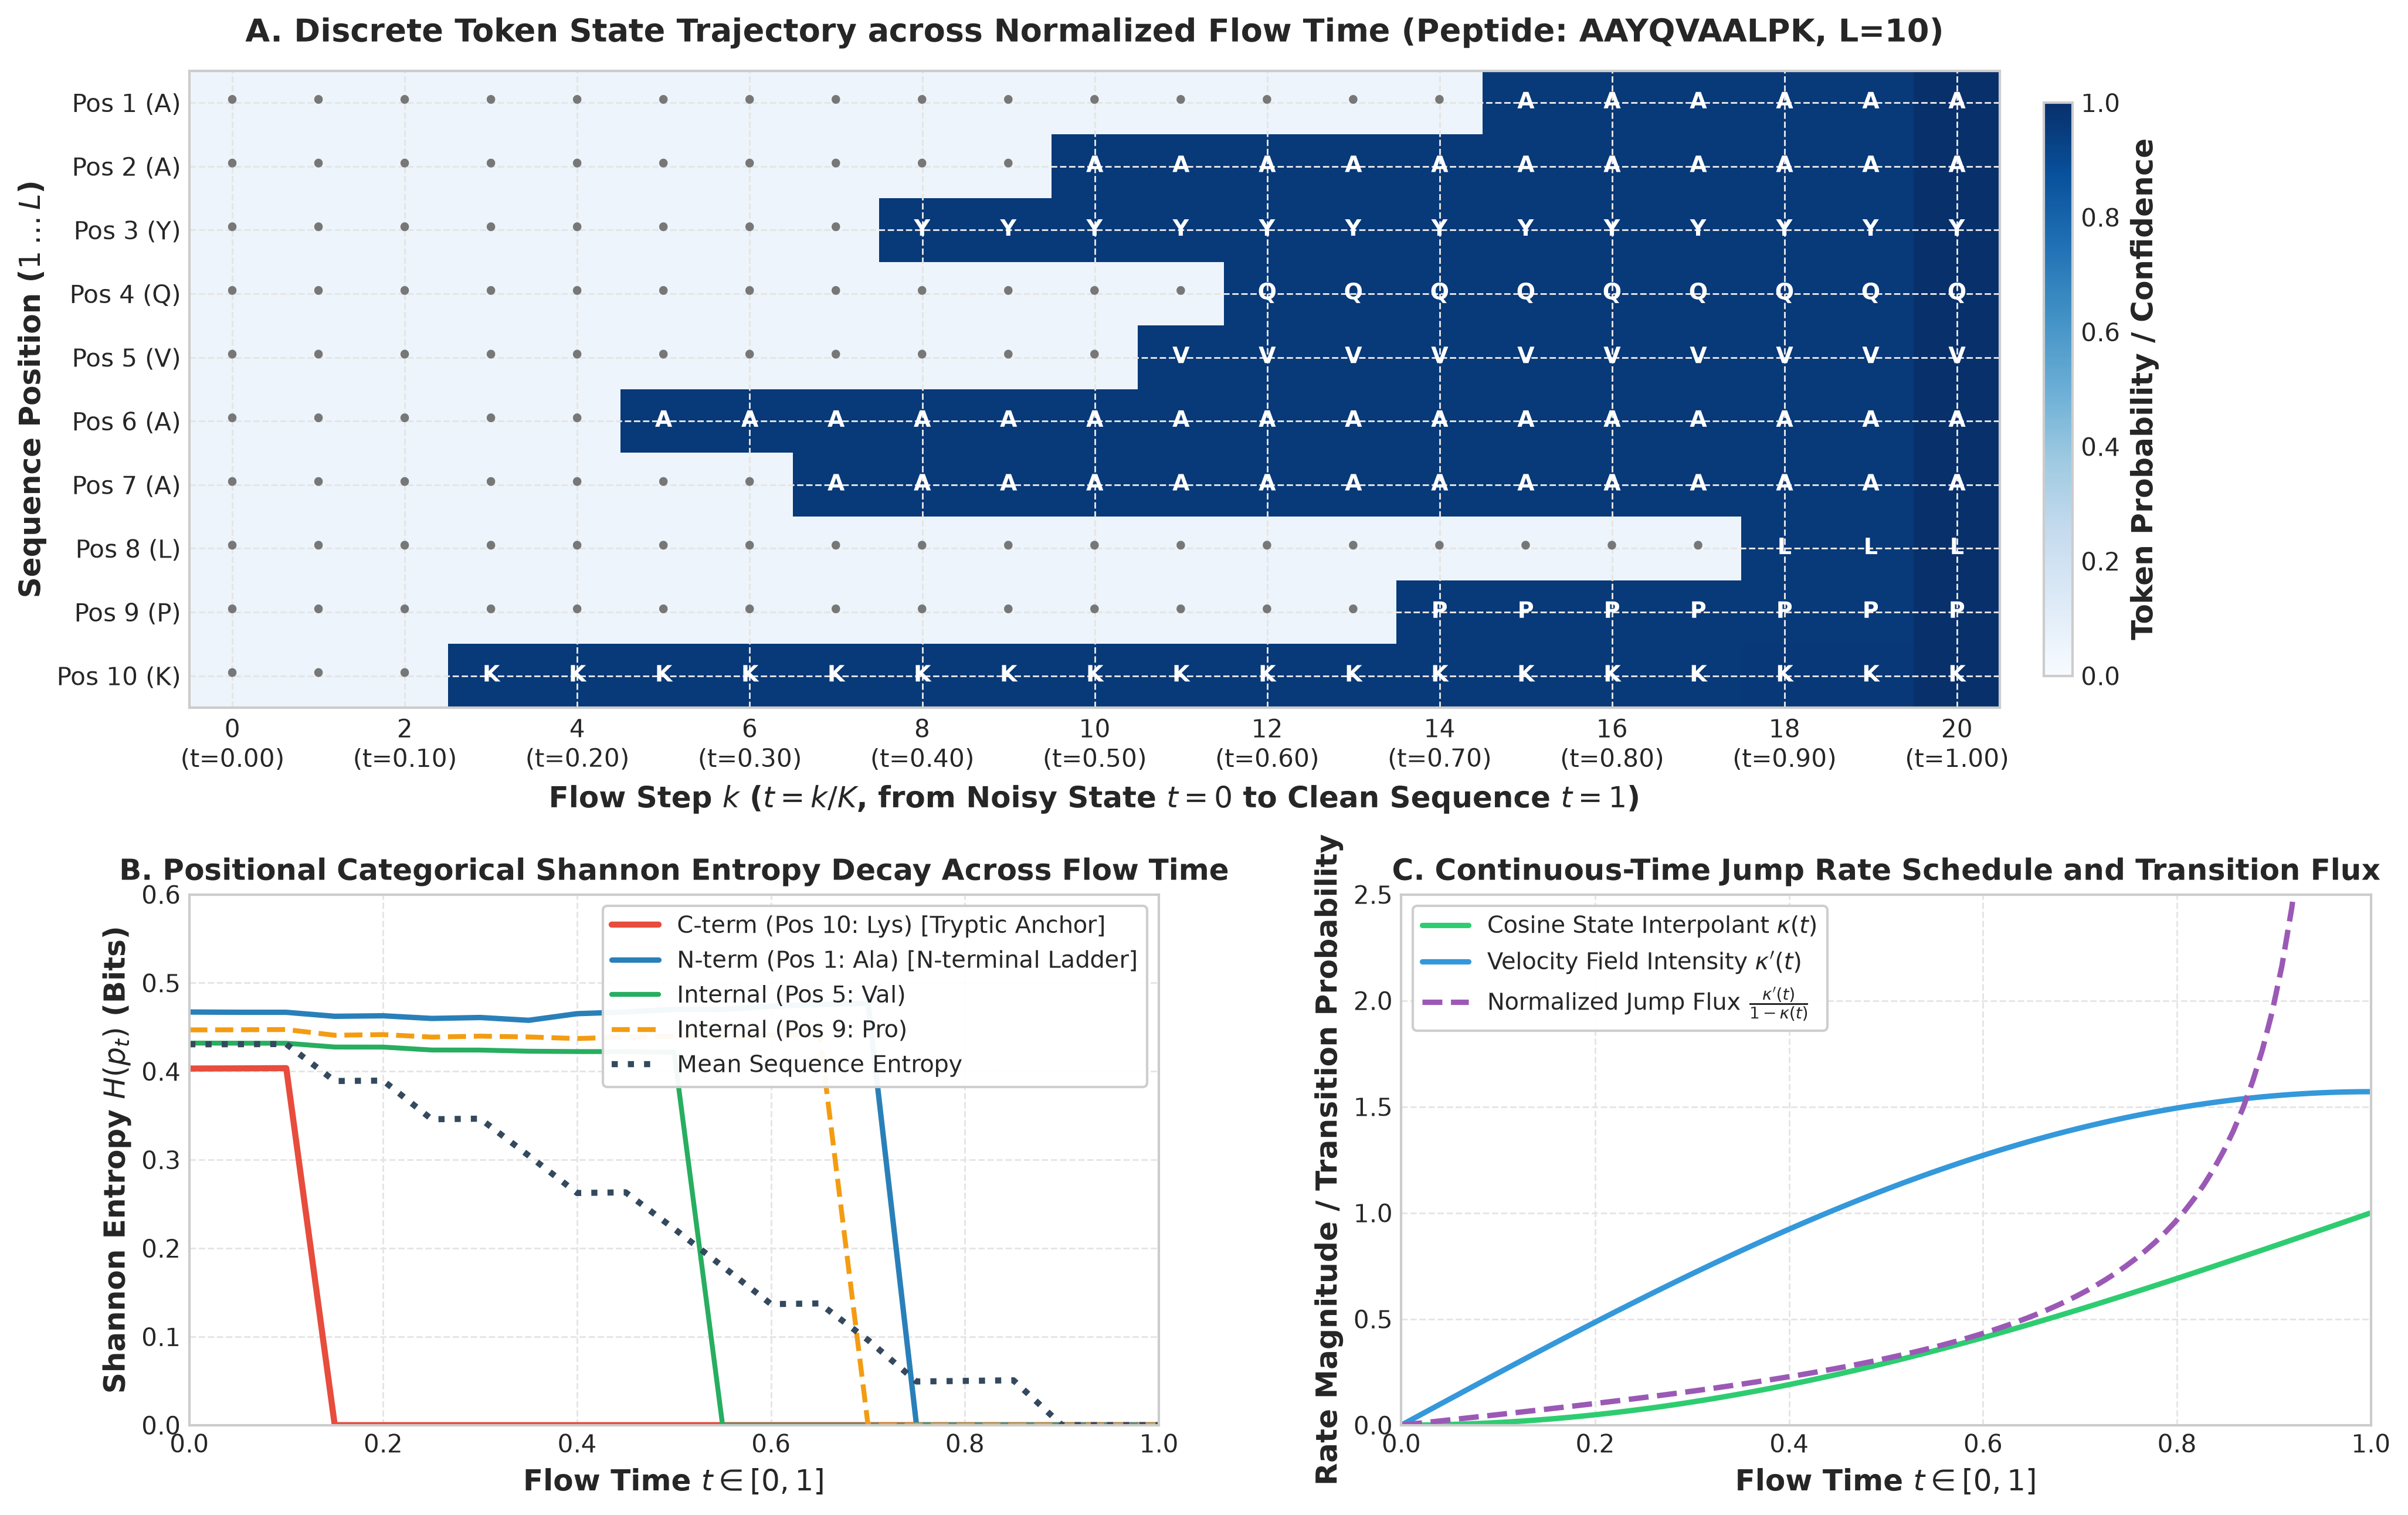
\includegraphics[width=0.88\textwidth]{images/ctmc_flow_dynamics.png}
\caption{Empirical verification of Continuous-Time Markov Chain (CTMC) flow dynamics evaluated across 10,000 biological spectra. (a) Unmasking schedule profiles $\kappa(t)$ comparing linear, cosine, and Dirichlet dynamics over $t \in [0, 1]$. (b) Positional categorical Shannon entropy decay across reverse flow sampling steps, showing progressive uncertainty reduction. (c) Token commitment velocity $\frac{\mathrm{d}\kappa}{\mathrm{d}t}$ across integration time. (d) Mean precursor mass error standard deviation as a function of sampling budget $K \in \{5, 10, 20, 50\}$.}
\label{fig:ctmc_flow_dynamics}
\end{figure}

As shown in Figure~\ref{fig:ctmc_flow_dynamics}, sequence entropy under the cosine schedule decreases smoothly across the 20 sampling steps, avoiding premature commitment to erroneous residues during early integration.

\section{Discrete Flow Matching Objective and Training Algorithm}

Because the exact posterior distribution $p_{1 \mid t}(x_1 \mid x_t, \mathcal{S})$ is intractable, we train a neural network $p_{1 \mid t}^\theta(x_1 \mid x_t, t, \mathcal{S})$ to predict clean peptide sequences $x_1$ conditioned on corrupted sequences $x_t$, continuous flow time $t$, and spectrum features $\mathcal{S}$ \citep{Campbell2024}.

\begin{defn}[Discrete Flow Matching Cross-Entropy Loss]
Given a dataset of paired spectra and peptide sequences $(x_1, \mathcal{S}) \sim p_{\text{data}}$, a time $t \sim \mathcal{U}[0, 1]$, and a corrupted sequence $x_t \sim p_{t \mid 1}(x_t \mid x_1)$, the DFlowNovo network parameterized by $\theta$ is optimized by minimizing:
\begin{equation}
\mathcal{L}_{\text{DFM}}(\theta) = - \mathbb{E}_{(x_1, \mathcal{S}) \sim p_{\text{data}}} \, \mathbb{E}_{t \sim \mathcal{U}[0, 1]} \, \mathbb{E}_{x_t \sim p_{t \mid 1}(x_t \mid x_1)} \left[ \frac{1}{\sum_{d=1}^D \mathbb{I}(x_t^d = [M])} \sum_{d: x_t^d = [M]} \log p_{1 \mid t}^\theta(x_1^d \mid x_t, t, \mathcal{S}) \right]
\label{eq:dfm_loss}
\end{equation}
\end{defn}

Notice that in Equation~\ref{eq:dfm_loss}, cross-entropy is evaluated exclusively over masked token positions ($x_t^d = [M]$), matching the simulation-free training recipe of \citet{Campbell2024}. Unmasked positions already match the ground-truth target under the canonical flow $R_t^*$ and require no gradient updates.

Algorithm~\ref{alg:ctmc_training} outlines the complete training procedure for DFlowNovo.

\begin{algorithm}[!ht]
\caption{Continuous-Time Discrete Flow Matching (CTMC) Training}
\label{alg:ctmc_training}
\begin{algorithmic}[1]
\Require Dataset of tandem spectra and ground-truth sequences $\mathcal{D} = \{(\mathcal{S}^{(n)}, Y^{(n)})\}_{n=1}^N$, schedule function $\kappa(t)$, batch size $B$, learning rate $\eta_{\text{lr}}$.
\Ensure Optimized model parameters $\theta = \{\theta_{\text{enc}}, \theta_{\text{dec}}, \theta_{\text{len}}\}$.
\State Initialize network parameters $\theta$ with AdaLN-Zero identity initialization ($W_{\text{ada}} = 0$).
\While{not converged}
    \State Sample a minibatch of $B$ spectrum-peptide pairs $\{(\mathcal{S}_b, x_{1, b})\}_{b=1}^B \sim \mathcal{D}$.
    \State Sample continuous flow times independently: $t_b \sim \mathcal{U}(0, 1)$ for $b \in \{1, \dots, B\}$.
    \State Compute unmasking probabilities: $\kappa_b = \kappa(t_b)$.
    \State Corrupt clean targets to generate $x_{t, b}$:
    \For{$b = 1$ \textbf{to} $B$}
        \For{position $d = 1$ \textbf{to} $D_b$}
            \State Sample $u \sim \mathcal{U}(0, 1)$.
            \State $x_{t, b}^d \gets \begin{cases} x_{1, b}^d & \text{if } u < \kappa_b \\ [M] & \text{if } u \ge \kappa_b \end{cases}$
        \EndFor
    \EndFor
    \State Compute spectrum encoder representations: $H_{\text{spec}, b} = \text{SpectrumEncoder}_{\theta}(\mathcal{S}_b)$.
    \State Predict length logits and clean residue probabilities:
    \State $\hat{p}_{\text{len}, b} = \text{LengthHead}_{\theta}(H_{\text{spec}, b}[CLS])$
    \State $\hat{p}_{1 \mid t, b} = \text{Decoder}_{\theta}(x_{t, b}, t_b, M_{\text{prec}, b}, z_b, H_{\text{spec}, b})$
    \State Compute length cross-entropy loss: $\mathcal{L}_{\text{len}} = - \frac{1}{B} \sum_{b=1}^B \log \hat{p}_{\text{len}, b}(D_b)$.
    \State Compute sequence flow loss over masked positions:
    \State $\mathcal{L}_{\text{seq}} = - \frac{1}{B} \sum_{b=1}^B \frac{1}{\sum_d \mathbb{I}(x_{t, b}^d = [M])} \sum_{d: x_{t, b}^d = [M]} \log \hat{p}_{1 \mid t, b}^d(x_{1, b}^d)$.
    \State Total objective: $\mathcal{L}_{\text{total}} = \mathcal{L}_{\text{seq}} + \lambda_{\text{len}} \mathcal{L}_{\text{len}}$.
    \State Compute gradients $\nabla_\theta \mathcal{L}_{\text{total}}$, clip norm to $1.0$, and update parameters via AdamW.
\EndWhile
\end{algorithmic}
\end{algorithm}
